\documentclass[a4paper]{article}

\usepackage{polski}
\usepackage[utf8]{inputenc}

\usepackage[export]{adjustbox}
\usepackage{scrextend}
\usepackage{amsfonts}
\usepackage{amsmath}
\usepackage{svg}


\usepackage{geometry}
\geometry{a4paper, left=15mm, top=30mm, right=15mm, bottom=20mm}

\usepackage{gensymb}
\usepackage{graphicx} 
\usepackage{isotope}
\usepackage{array}
\usepackage{float}
\usepackage{titlesec}
\usepackage{fancyhdr}
\usepackage{multirow}

\usepackage{hyperref}
\usepackage{sectsty}
\usepackage{enumitem}
\usepackage{listings}
\usepackage[labelformat=simple]{subcaption}
\usepackage{xcolor,colortbl}
\usepackage{animate}

\sectionfont{\normalfont\huge\sectionrule{0pt}{0pt}{-6pt}{1pt}}
\subsectionfont{\normalfont\LARGE}

\pagestyle{fancy}
\fancyhf{}
\fancyhead[LE,LO]{\Large Łukasz Kwinta}
\fancyhead[LE,RO]{\Large Laboratorium 4 - Wyznaczanie przecięć odcinków}
\fancyfoot[CE,CO]{\Large\thepage}

\renewcommand{\footrulewidth}{1pt}
\renewcommand{\headrulewidth}{1pt}

\definecolor{Gray}{gray}{0.85}
\definecolor{LightGray}{gray}{0.95}

\newcolumntype{a}{>{\columncolor{Gray}}c}
\newcolumntype{b}{>{\columncolor{white}}c}

\hypersetup{
    colorlinks,
    citecolor=black,
    filecolor=black,
    linkcolor=black,
    urlcolor=black
}

\title{\fontsize{30pt}{30pt}\selectfont Laboratorium 4 \\ Wyznaczanie przecięć odcinków}
\author{\fontsize{20pt}{20pt}\selectfont Łukasz Kwinta}
\date{}

\begin{document}
\maketitle
\Large
\vspace*{\fill}
\section{Dane Techniczne}
Procesor: AMD Ryzen 7 5700U\\
System operacyjny: Ubuntu 20.04 w środowisku WSL 2 na Windows 11 x64\\
Pamięć ram: 32 GB DDR4\\
\\
\\
Środowisko i język: Python 3.9 + Jupyter Notebook w środowisku Anaconda\\
Wykresy tworzyłem przy pomocy narzędzia przygotowanego przez KN Bit, 
do obliczeń numerycznych używałem biblioteki numpy.
 Dane przechowywałem w zmiennych typu float – typ danych o rozmiarze 64 bitów, 
 odpowiednik typu double w języku C.
\pagebreak
\section{Opis Realizacji Ćwiczenia}
Celem ćwiczenia była implementacja algorytmu wyznaczającego przecięcia wszystkich odcinków
na płaszczyźnie za pomocą algorytmu zamiatania.

\subsection{Generowanie zbiorów testowych}
    Pierwszym krokiem realizacji ćwiczenia było przygotowanie funkcji generujacej losowe odcinki 
    na płaszczyźnie. Wykorzystałem w tym celu funkcję wbudowaną w pakiety Pythona \verb|random.random.uniform()|
    losującą floaty w zadanym przedziale. Gdy jakiś punkt wylosowany został pionowo to przesuwałem jeden jego koniec -
    aby zbiór danych nie zawierał pionowych odcinków.\\
    Wygenerowany zbiór miał zawierać $20$ odcinków w końcach o współrzędnych w przedziałach $\large x \in \langle 0,1000 \rangle$ oraz $\large y \in \langle 0,1000\rangle$
    \begin{figure}[H]
        \centering
        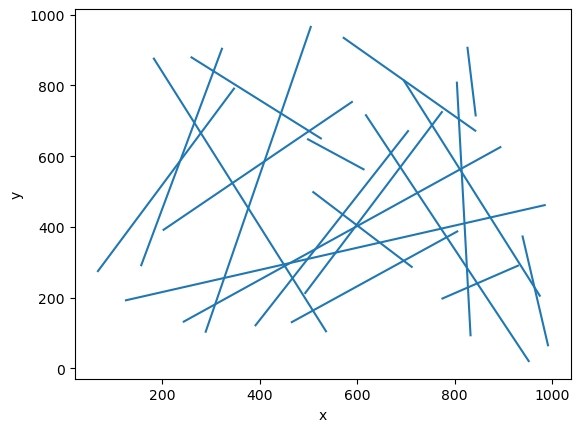
\includegraphics{wizualizacje/random_segments.png}
        \label{fig:random_segments}
        \caption{Wizualizacja przykładowego zbioru wygenerowanych odcinków}
    \end{figure}

\subsection{Sprawdzenie czy w zbiorze prostych istnieje przecięcie}
    Kolejnym krokiem było zaimplementowanie uproszczonej wersji algorytmu który, kończy działanie w momencie 
    znalezienia pierwszych prostych które się przecinają. Do reprezentacji struktury stanu i struktury zdarzeń
    użyłem \verb|SortedSet| z bibliotek \verb|sortedcontainters| który jest realizacją drzewa BST 
    pozwala dodawać i wyjmować elementy z drzewa w czasie logarytmicznym, oraz sprawdzanie ich poprzedników 
    i następników.\\
    Aby w łatwy sposób aktualizować kolejność odcinków w strukturze zdarzeń zaimplementowałem klasę reprezentującą
    odcinek w której zdefiniowałem własny operator porównania które oblicza wartość $y$ danego odcinka dla danego $x$,
    oraz wykorzystałem statyczne pole do ustalania $x$ aby wszystkie odcinki były porównywane w tym samym $x$. 
    Wartość $x$ aktualizuję podczas przetwarzania każdego zdarzenia.\\
    \\
    Poniżej krótka lista kroków pokazująca działanie algorytmu:
    
    \begin{enumerate}
        \item Wstawienie krańców wierzchołków do struktury zdarzeń $Q$ w porządku względem rosnących współrzędnych $x$
        \item Dopóki są zdarzenia w $Q$:
            \begin{enumerate}
                \item Pobranie pierwsze zdarzenie z $Q$
                \item Jeśli zdarzenie jest początkiem odcinka:
                    \begin{enumerate}
                        \item Aktualizacja obecnego $x$ do porównania odcinków 
                        \item Dodanie odcinka do struktury stanu $T$
                        \item Jeśli odcinek przecina się z poprzednikiem lub następnikiem: Znaleziono przecięcie
                    \end{enumerate}
                \item Jeśli zdarzenie jest końcem odcinka:
                    \begin{enumerate}
                        \item Aktualizacja obecnego $x$ do porównania odcinków 
                        \item Usunięcie odcinka który kończy ze struktury $T$
                    \end{enumerate}
            \end{enumerate}
        \item Koniec algorytmu - brak przecięcia
    \end{enumerate}

    Do sprawdzanie przecięć użyłem prostego algorytmu korzystającego z wyznaczników. Na początek obliczyłem 
    znaki 4 wyznaczników między odcinkami, a końcami drugiego odcinka korzystając z własnej funkcji znaku:
    \[
        sgn = \left\{ 
            \begin{array}{ll}
                1 & \mbox{jeśli } x > \varepsilon \\
                -1 & \mbox{jeśli } x < -\varepsilon \\
                0 & \mbox{w pozostałych przypadkach}
            \end{array}
        \right. 
    \]

    dla $\varepsilon = 10^{-12}$. A następnie jeśli znak któregoś wyznacznik był 0 to znaczy, że punkty które reprezentował
    są współliniowe, a więc koniec jednego z odcinków zawiera się w drugim. Na koniec sprawdzam, czy wyznaczniki są
    przeciwnych znaków, tzn. punkty sprawdzane leżą po przeciwnych stronach odcinka, z czego wynika, że istnieje przecięcie.
    \\\\
    Jeśli już wiem, że przecięcie istnieje mogę wyznaczyć przecięcie korzystając z układu równań kierunkowych odcinku
    rozwiązanego metodą macierzy. Jeśli:
    \[s_1: y = a_1x+b_1\]
    \[s_2: y = a_2x+b_2\]
    to punkt przecięcia $P = (x_P, y_P)$ ma wtedy współrzędne w następującym miejscu:
    \[
        x_P = \frac{b_1 - b_2}{a_2 - a_1}
        \qquad \qquad
        y_P = \frac{a_2b_1 - a_1b_2}{a_2 - a_1}
    \]  

\subsection{Wizualizacja działania algorytmu sprawdzającego przecięcie}
    Zmodyfikowałem powyższy program tak aby generował animację z przebiegiem algorytmu. Przyjąłem następujące
    oznaczenia:
    \begin{itemize}
        \item Zielona prosta i zielony punkt - prosta wizualizuję miotłę, a punkt oznacza konkretny punkt zdarzenia który jest rozważany
        \item Żółte proste - proste znajdujące się w strukturze stanu $T$
        \item Czerwone proste - proste obecnie sprawdzane pod kątem przecinania się 
        \item Fioletowy punkt - znaleziony punkt przecięcia 
    \end{itemize}
    Poniżej zawarłem plik z animacją pokazujące kolejne kroki działania algorytmu oraz jego stan końcowy.
    \textbf{\textit{Uwaga! Animacja może nie działać w każdym
    programie do plików PDF, została przetestowana w programie Adobe Acrobat gdzie działa.
    W razie gdyby animacja nie działała będzie wyświetlona jedna klatka animacji. Samą 
    animację można znaleźć w notebooku z rozwiązaniem zadania.}}

    \begin{figure}[H]
        \centering
        \animategraphics[width=.8\textwidth, loop, autoplay, poster=29]{5}
        {wizualizacje/animation_is_intersect/is_intersect_animation-}{0}{88}
        \caption{Animacja działania algorytmu dla przykładowego zbioru odcinków}
        \label{fig:is_intersect_animation}
    \end{figure}

    \begin{figure}[H]
        \centering
        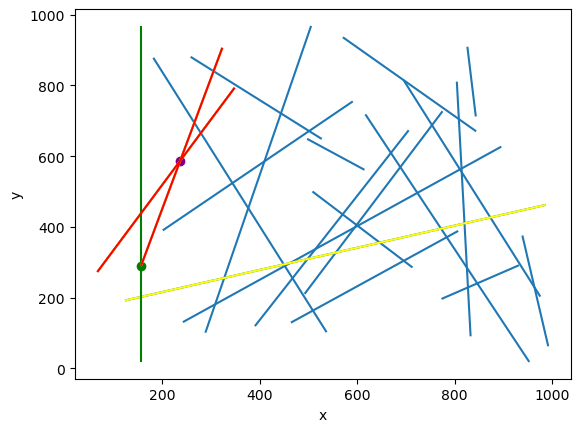
\includegraphics[width=.8\textwidth]{wizualizacje/is_intersect_random.png}
        \label{fig:is_intersect_res_random}
        \caption{Stan końcowy działania algorytmu dla losowo wygenerowanych odcinków}
    \end{figure}

\subsection{Algorytm wykrywający wszystkie przecięcia}
Końcowym elementem wykonania zadania było stworzenie algorytmu który wykrywa wszystkie przecięcia w zbiorze 
prostych. Do realizacji struktury zdarzeń $Q$ i struktury stanu $T$, użyłem \verb|SortedSet| tak samo jak wcześniej
lecz dla wygody zdarzenia musiałem opakować w obiekty klasy \verb|Event| którą przygotowałem, dzięki nim 
wiem co oznacza dane zdarzenie i mogę przekazywać argumenty ze zdarzenia do zdarzenia.\\
Główną zmianą w strukturach danych była dodatkowa struktura zbioru \verb|set()| realizowanego jako 
hash set, do sprawdzania które przecięcia zostały już dodane do struktury zdarzeń aby nie dodawać wielokrotnie
tych samych przecięć do struktury zdarzeń. \\
Do zamiany punktów w strukturze stanu w momencie wykrywania przecięć wykorzystałem przygotowany mechanizm 
do ustalania $x$. Najpierw usuwam odcinki ze struktury stanu, następnie jako obecną wartość $x$ ustawiam 
współrzędną $x$ przecięcia które analizuję przesuniętą o $\varepsilon = 10^{-12}$.\\
Poniżej przedstawiam uproszczony schemat działania algorytmu:

\begin{enumerate}
    \item Wstawienie krańców wierzchołków do struktury zdarzeń $Q$ w porządku względem rosnących współrzędnych $x$
    \item Dopóki są zdarzenia w $Q$:
        \begin{enumerate}
            \item Pobranie pierwsze zdarzenie z $Q$
            \item Jeśli zdarzenie jest początkiem odcinka:
                \begin{enumerate}
                    \item Aktualizacja obecnego $x$ do porównania odcinków 
                    \item Dodanie odcinka do struktury stanu $T$
                    \item Jeśli odcinek przecina się z poprzednikiem lub następnikiem
                    \begin{enumerate}
                        \item Sprawdzenie czy przecięcie jest w zbiorze przecięć
                        \item Jeśli nie to dodanie przecięcia do $Q$
                        \item Dodanie przecięcia do zbioru przecięć
                    \end{enumerate}
                \end{enumerate}
            \item Jeśli zdarzenie jest końcem odcinka:
                \begin{enumerate}
                    \item Aktualizacja obecnego $x$ do porównania odcinków 
                    \item Jeśli poprzednik i następnik odcinka się przecinają:
                    \begin{enumerate}
                        \item Sprawdzenie czy przecięcie jest w zbiorze przecięć
                        \item Jeśli nie to dodanie przecięcia do $Q$
                        \item Dodanie przecięcia do zbioru przecięć
                    \end{enumerate}
                    \item Usunięcie odcinka który kończy ze struktury $T$
                \end{enumerate}
            \item Jeśli zdarzenie jest przecięciem
                \begin{enumerate}
                    \item Niech $s_1$ i $s_2$ to odcinki które przecinają się w sprawdzanym punkcie $(x_P, y_P)$
                    \item Usunięcie $s_1$ i $s_2$ ze struktury stanu $T$
                    \item Aktualizacja obecnego $x$ do porównania odcinków jako $x := x_P + \varepsilon$
                    \item Dodanie $s_1$ i $s_2$ do struktury stanu $T$
                    \item Jeśli nowy sąsiad $s_1$ i $s_1$ się przecinają:
                    \begin{enumerate}
                        \item Sprawdzenie czy przecięcie jest w zbiorze przecięć
                        \item Jeśli nie to dodanie przecięcia do $Q$
                        \item Dodanie przecięcia do zbioru przecięć
                    \end{enumerate}
                    \item Jeśli nowy sąsiad $s_2$ i $s_2$ się przecinają:
                    \begin{enumerate}
                        \item Sprawdzenie czy przecięcie jest w zbiorze przecięć
                        \item Jeśli nie to dodanie przecięcia do $Q$
                        \item Dodanie przecięcia do zbioru przecięć
                    \end{enumerate}
                \end{enumerate}
        \end{enumerate}
    \item Zwrócenie listy przecięć
\end{enumerate}

Przecięcia są sprawdzane i obliczane za pomocą tych samych funkcji co w poprzednim algorytmie.

\subsection{Wizualizacja algorytmu wykrywającego wszystkie przecięcia}
Wizualizację algorytmu przygotowałem podobnie jak w przypadku algorytmu sprawdzającego jedno przecięcie,
wszystkie oznaczenia są identyczne. Podobnie jak wcześniej poniżej zawieram przykładową animację oraz 
efekt końcowy działania algorytmu dla losowo wygenerowanego zbioru odcinków.

\begin{figure}[H]
    \centering
    \animategraphics[width=.8\textwidth, loop, autoplay, poster=38]{5}
    {wizualizacje/animation_find_intersect/find_intersect_animation-}{0}{90}
    \caption{Animacja działania algorytmu dla przykładowego zbioru odcinków}
    \label{fig:find_intersect_animation}
\end{figure}

\begin{figure}[H]
    \centering
    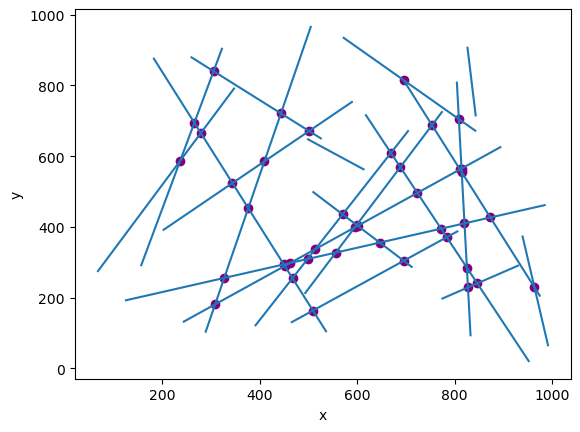
\includegraphics[width=.8\textwidth]{wizualizacje/find_intersect_random.png}
    \label{fig:find_intersect_res_random}
    \caption{Stan końcowy działania algorytmu dla losowo wygenerowanych odcinków}
\end{figure}

\section{Testy}
\subsection{Testy algorytmu szukającego jednego przecięcia}
Wyróżniłem tutaj dwa przypadki szczególne które warto zawrzec w sprawozdaniu, więcej testów
można obejrzeć w załączonym notebooku.\\\\
Pierwszym szczególnym przypadkiem to znalezienie przecięcia znajdującego się na końcu zbioru:\\

\begin{figure}[H]
    \centering
    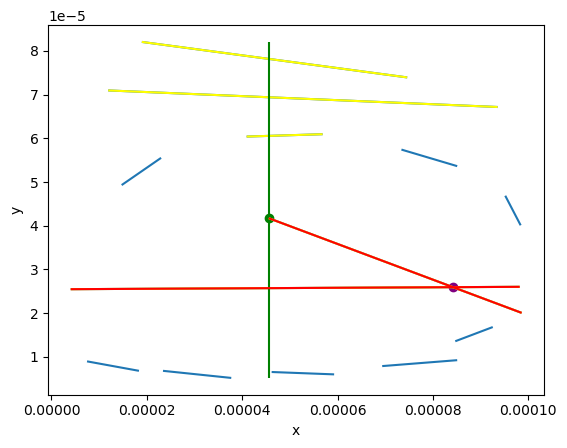
\includegraphics[width=\textwidth]{wizualizacje/is_random_edge_case_1.png}
    \label{fig:is_intersect_random_edgecase_1}
    \caption{Wizualizacja wyniku szukania przecięć dla pierwszego szczególnego przypadku}
\end{figure}

Drugim szczególnym przypadkiem to upewnienie się, że w gęstym zbiorze odcinków algorytm nie znajdzie,
żadnego przecięcia:
\begin{figure}[H]
    \centering
    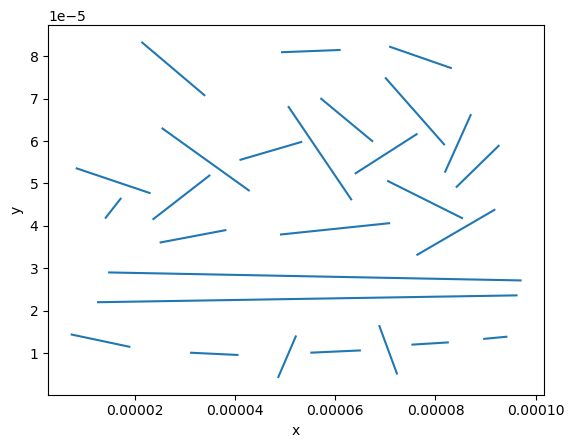
\includegraphics[width=\textwidth]{wizualizacje/is_random_edge_case_2.png}
    \label{fig:is_intersect_random_edgecase_2}
    \caption{Wizualizacja wyniku szukania przecięć dla pierwszego szczególnego przypadku}
\end{figure}

\subsection{Testy algorytmu szukającego wszystkich przecięć}
Przy testowaniu tego algorytmu główną trudnością były gęste zbiory odcinków dlatego zawarłem jeden taki 
przypadek w sprawozdaniu:
\begin{figure}[H]
    \centering
    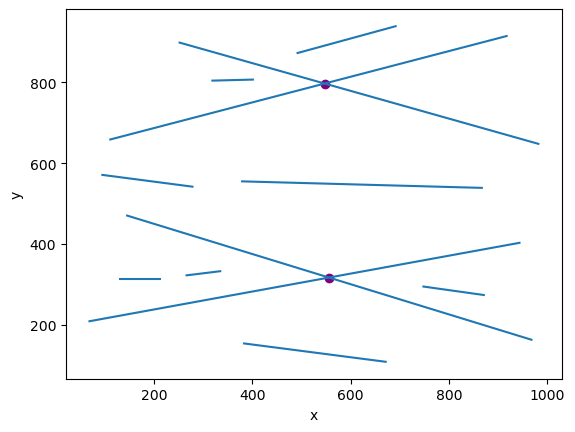
\includegraphics[width=\textwidth]{wizualizacje/find_random_edge_case_1.png}
    \label{fig:find_intersect_random_edgecase_1}
    \caption{Wizualizacja wyniku szukania przecięć dla pierwszego szczególnego przypadku}
\end{figure}

Kolejnym ciekawym przypadkiem jest sprawdzenie czy algorytm poprawnie radzi sobie ze sprawdzaniem 
duplikatów, poniżej zamieszczam wynik działania algorytmu dla takiego testu. Test ten powoduje
wielokrotne dodawanie tego samego przecięcia ponieważ jest kilka odcinków nie przecinających się 
między przecinającymi się odcinkami, a więc przy usuwaniu tychże odcinków sprawdzamy wiele 
razy te same przecinające się proste:

\begin{figure}[H]
    \centering
    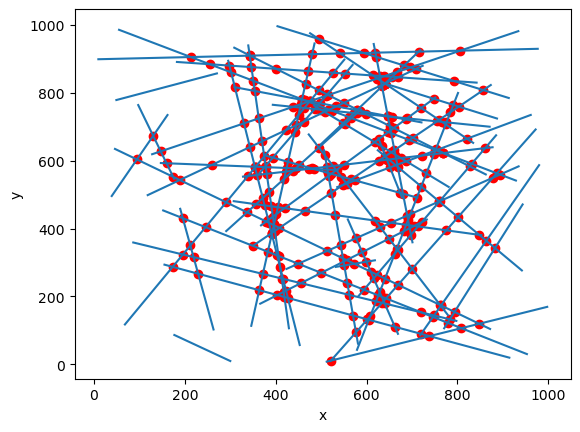
\includegraphics[width=.8\textwidth]{wizualizacje/find_random_edge_case_2.png}
    \label{fig:find_intersect_random_edgecase_2}
    \caption{Wizualizacja wyniku szukania przecięć dla drugiego szczególnego przypadku}
\end{figure}

\section{Wnioski}
Na podstawie swoich testów mogę stwierdzić, że algorytmy działają poprawnie. Nie udało mi się wygenerować 
przypadków które nie działałyby poprawnie. Użycie \verb|SortedSet| do struktur zdarzeń pozwoliło 
zaimplementować algorytm o odpowiedniej złożoności oraz pozwoliło zaoszczędzić czas na implementowanie
własnego drzewa BST. Użycie hashset pozwoliło w drugim algorytmie umożliwiło skuteczne wykrywanie
duplikatów przecięć w złożoności stałej.

\end{document}